\documentclass{bioinfo}
\copyrightyear{2014}
\pubyear{2014}
%\firstpage{1}
%


\usepackage{hyperref}



\begin{document}
\firstpage{1}

%\title[short Title]{Structure prediction of globular proteins using predicted residue contacts.}
%\title[short Title]{PconsFold: ab-initio protein folding using Rosetta and predicted residue contacts.}
\title[PconsFold]{PconsFold: Improved contact predictions improve
  protein models}
%\title[short Title]{Advancement in residue contact prediction improves quality of predicted structural models.}
%\author[Sample \textit{et~al}]{Mirco Michel\,$^{1,2}$, Marcin J. Skwark\,$^{3}$ and Arne Elofsson\,$^{1,2}$\footnote{to whom correspondence should be addressed}}
\author[M.Michel \textit{et~al}]{Mirco Michel\,$^{1,2}$, Sikander
  Hayat\,$^{3}$, Marcin Skwark\,$^{4}$, Chris Sander\,$^{5}$, Debora
  S. Marks\,$^{3}$,  and Arne Elofsson\,$^{1,2,}$\footnote{To whom correspondence should be addressed.}}
\address{$^{1}$Department of Biochemistry and Biophysics, Stockholm University, 10691 Stockholm, Sweden,
$^{2}$Science for Life Laboratory, Box 1031, 17121 Solna, Sweden,
$^{3}$Department of Systems Biology, Harvard Medical School, Boston, Massachusetts, USA,
$^{4}$Department of Information and Computer Science, Aalto University, PO Box 15400, FI-00076 Aalto, Finland, and
$^{5}$Computational Biology Center, Memorial Sloan-Kettering Cancer Center, New York, New York, USA}

\history{Received on XXXXX; revised on XXXXX; accepted on XXXXX}

\editor{Associate Editor: XXXXXXX}

\maketitle

\begin{figure*}[!b]%figure1
\centerline{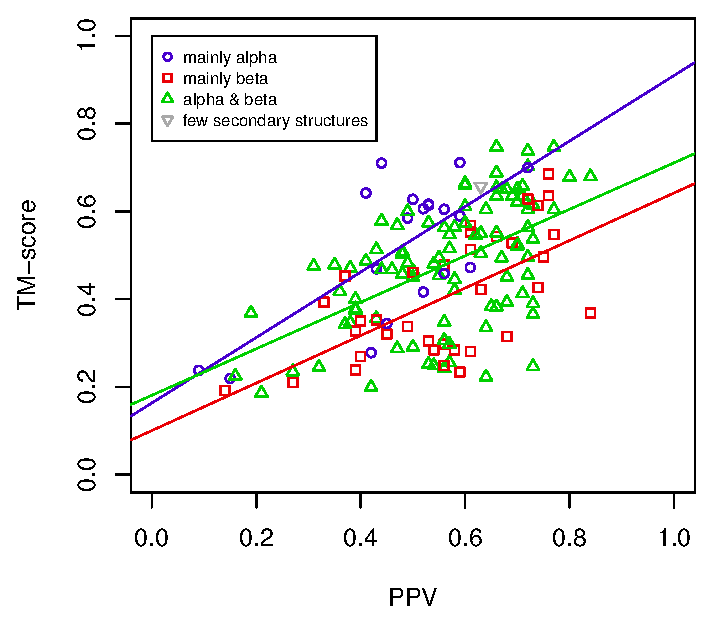
\includegraphics[scale=0.7]{figures/TMscore_EVfold-pcons_vs_PPV-plmDCA.eps}}
\caption{PPV vs. TM-score for EVfold-PLM on the PSICOV dataset. It
shows the same trend as with PconsFold: alpha-helical proteins seem to
be easier to fold than beta-sheet containing proteins.}\label{fig:ppvtm_evfold}
\end{figure*}


\section{Supplementary material}
\begin{table*}[!t]
\processtable{PSICOV dataset of 150 proteins. Proteins from the small subset are marked with *. \label{tab:psicovset}}
{\begin{tabular}{lllllllll}\toprule
    PDB ID & Uniprot ID   & Sequence length & PDB ID & Uniprot ID   & Sequence length & PDB ID & Uniprot ID   & Sequence length \\ \midrule
    1A3A *  & PTM3C\_ECOLI & 148             & 1GBS   & LYG\_CYGAT   & 185             & 1M4J   & TWF1\_MOUSE  & 142             \\
    1A6M   & MYG\_PHYCD   & 151             & 1GMI   & KPCE\_RAT    & 136             & 1M8A   & CCL20\_HUMAN & 70              \\
    1A70   & FER1\_SPIOL  & 97              & 1GMX   & C6EFE9\_ECOBD & 108             & 1MK0   & TEV1\_BPT4   & 97              \\
    1AAP   & A4\_HUMAN    & 58              & 1GUU   & MYB\_MOUSE   & 52              & 1MUG   & MUG\_ECOLI   & 168             \\
    1ABA   & GLRX\_BPT4   & 87              & 1GZ2   & OC17\_CHICK  & 142             & 1NB9   & RIFK\_HUMAN  & 147             \\
    1AG6   & PLAS\_SPIOL  & 99              & 1GZC   & LEC\_ERYCG   & 239             & 1NE2   & Q9HIL9\_THEAC & 200             \\
    1AOE   & DYR\_CANAX   & 192             & 1H0P   & CYP5\_CAEEL  & 182             & 1NPS   & DESS\_MYXXA  & 88              \\
    1ATL   & VM1AD\_CROAT & 202             & 1H2E   & Q9ALU0\_GEOSE & 207             & 1NRV   & GRB10\_HUMAN & 105             \\
    1ATZ *  & VWF\_HUMAN   & 189             & 1H4X   & SP2AA\_LYSSH & 117             & 1NY1   & PDAA\_BACSU  & 240             \\
    1AVS   & TNNC2\_CHICK & 90              & 1H98   & FER\_THET8   & 78              & 1O1Z *  & Q9X1V6\_THEMA & 234             \\
    1BDO *  & BCCP\_ECOLI  & 80              & 1HDO *  & BLVRB\_HUMAN & 206             & 1P90   & Q9F5X9\_AZOVI & 145             \\
    1BEB   & LACB\_BOVIN  & 162             & 1HFC   & MMP1\_HUMAN  & 169             & 1PCH   & PTHP\_MYCCT  & 88              \\
    1BEH   & PEBP1\_HUMAN & 187             & 1HH8   & NCF2\_HUMAN  & 213             & 1PKO   & MOG\_RAT     & 139             \\
    1BKR   & SPTB2\_HUMAN & 109             & 1HTW   & TSAE\_HAEIN  & 158             & 1QF9   & KCY\_DICDI   & 194             \\
    1BRF   & RUBR\_PYRFU  & 53              & 1HXN   & HEMO\_RABIT  & 219             & 1QJP   & OMPA\_ECOLI  & 171             \\
    1BSG   & BLAC\_STRAL  & 266             & 1I1J   & MIA\_HUMAN   & 108             & 1QL0   & NUCA\_SERMA  & 241             \\
    1C44   & NLTP\_RABIT  & 123             & 1I1N   & PIMT\_HUMAN  & 226             & 1R26   & Q9NG23\_TRYBB & 125             \\
    1C52   & CY552\_THETH & 131             & 1I4J   & RL22\_THETH  & 110             & 1ROA   & CYTD\_HUMAN  & 122             \\
    1C9O   & CSPB\_BACCL  & 66              & 1I58   & CHEA\_THEMA\_2 & 189             & 1RW1   & Q9HXX5\_PSEAE & 114             \\
    1CC8   & ATX1\_YEAST  & 73              & 1I5G   & O77093\_CRIFA & 144             & 1RW7   & HSP31\_YEAST & 243             \\
    1CHD *  & CHEB\_SALTY  & 203             & 1I71   & APOA\_HUMAN  & 83              & 1RYB   & CRS2\_MAIZE  & 205             \\
    1CJW   & SNAT\_SHEEP  & 166             & 1IHZ *  & NUC\_STAAU   & 149             & 1SMX   & RNE\_ECOLI   & 96              \\
    1CKE   & KCY\_ECOLI   & 227             & 1IIB   & PTQB\_ECOLI  & 106             & 1SVY   & SEVE\_DICDI  & 114             \\
    1CTF   & RL7\_ECOLI   & 74              & 1IM5 *  & O58727\_PYRHO & 180             & 1T8K   & ACP\_ECOLI   & 77              \\
    1CXY   & CYB5\_ECTVA  & 90              & 1IWD   & ERVB\_TABDI  & 215             & 1TIF   & IF3\_GEOSE   & 78              \\
    1CZN   & FLAV\_SYNE7  & 169             & 1J3A   & RL13\_PYRHO  & 142             & 1TQG   & CHEA\_THEMA  & 105             \\
    1D0Q   & PRIM\_GEOSE  & 103             & 1JBE   & CHEY\_ECOLI  & 128             & 1TQH *  & EST\_GEOSE   & 247             \\
    1D1Q   & PPAL\_YEAST  & 161             & 1JBK   & CLPB\_ECOLI  & 195             & 1TZV   & NUSB\_THEMA  & 142             \\
    1D4O   & NNTM\_BOVIN  & 184             & 1JFU   & TLPA\_BRAJA  & 186             & 1VFY   & VPS27\_YEAST & 73              \\
    1DBX   & YBAK\_HAEIN  & 158             & 1JFX   & LYSM1\_STRGL & 217             & 1VHU   & Y1521\_ARCFU & 211             \\
    1DIX   & RNLE\_SOLLC  & 208             & 1JKX   & PUR3\_ECOLI  & 212             & 1VJK   & Q8U3C7\_PYRFU & 98              \\
    1DLW   & TRHBN\_PARCA & 116             & 1JL1   & RNH\_ECOLI   & 155             & 1VMB   & RS6\_THEMA   & 140             \\
    1DMG   & RL4\_THEMA   & 225             & 1JO0   & Y1333\_HAEIN & 98              & 1VP6 *  & CNGK1\_RHILO & 138             \\
    1DQG   & MRC1\_MOUSE  & 135             & 1JO8 *  & ABP1\_YEAST  & 58              & 1W0H   & ERI1\_HUMAN  & 204             \\
    1DSX   & KCNA2\_RAT   & 87              & 1JOS   & RBFA\_HAEIN  & 128             & 1WHI   & RL14\_GEOSE  & 122             \\
    1EAZ   & PKHA1\_HUMAN & 125             & 1JVW   & MIP\_TRYCR   & 167             & 1WJX   & SSRP\_THET8  & 122             \\
    1EJ0   & RLME\_ECOLI  & 180             & 1JWQ *  & Q9LCR3\_PAEPO & 179             & 1WKC   & Q5SHW9\_THET8 & 184             \\
    1EJ8   & CCS1\_YEAST  & 140             & 1JYH   & SBMC\_ECOLI  & 157             & 1XDZ   & RSMG\_BACSU  & 240             \\
    1EK0   & VPS21\_YEAST & 170             & 1K6K   & CLPA\_ECOLI  & 143             & 1XFF   & GLMS\_ECOLI  & 240             \\
    1F6B   & SAR1B\_CRIGR & 198             & 1K7C   & RHA1\_ASPAC  & 233             & 1XKR   & CHEC\_THEMA  & 206             \\
    1FCY   & RARG\_HUMAN  & 236             & 1K7J   & YCIO\_ECOLI  & 206             & 2ARC   & ARAC\_ECOLI  & 164             \\
    1FK5   & NLTP\_MAIZE  & 93              & 1KID   & CH60\_ECOLI  & 203             & 2CUA *  & COX2\_THETH  & 135             \\
    1FL0   & AIMP1\_HUMAN & 171             & 1KQ6   & NCF1\_HUMAN  & 141             & 2HS1   & Q7SSI0\_9HIV1 & 99              \\
    1FNA   & FINC\_HUMAN  & 91              & 1KQR   & VP4\_ROTRH   & 179             & 2MHR   & HEMTM\_THEHE & 118             \\
    1FQT *   & BPHF\_BURXL  & 112             & 1KTG   & AP4A\_CAEEL  & 138             & 2PHY   & PYP\_HALHA   & 125             \\
    1FVG   & MSRA\_BOVIN  & 199             & 1KU3   & SIGA\_THEAQ  & 73              & 2TPS   & THIE\_BACSU  & 227             \\
    1FVK   & DSBA\_ECOLI  & 189             & 1KW4   & PHP\_DROME   & 89              & 2VXN   & TPIS\_LEIME  & 251             \\
    1FX2   & CY41\_TRYBB  & 235             & 1LM4   & DEF\_STAAU   & 194             & 3BOR   & IF4A2\_HUMAN & 237             \\
    1G2R   & Q97S59\_STRPN & 100             & 1LO7   & 4HBT\_PSEUC  & 141             & 3DQG   & HSP7F\_CAEEL & 151             \\
    1G9O   & NHRF1\_HUMAN & 91              & 1LPY   & LYS\_BPT4    & 164             & 5PTP   & TRY1\_BOVIN  & 223             \\ \botrule
\end{tabular}}{}
\end{table*}


\begin{table*}[!t]
\processtable{Dataset of 15 proteins from the EVfold publication. \label{tab:evfoldset}}
{\begin{tabular}{llll}\toprule
    PDB ID & Uniprot ID   & Sequence length & Sequence \\\midrule
    1BKR   & SPTB2\_HUMAN & 102 & KDALLLWCQMKTAGYPNVNIHNFTTSWRDGMAFNALIHKHRPDLIDFDKLKKSNAHYNLQ \\
	~&~&~& NAFNLAEQHLGLTKLLDPEDISVDHPDEKSIITYVVTYYHYF \\
    1E6K   & CHEY\_ECOLI  & 114 & FLVVDDFSTMRRIVRNLLKELGFNNVEEAEDGVDALNKLQAGGYGFVISDWNMPNMDGLE \\
	~&~&~& LLKTIRADGAMSALPVLMVTAEAKKENIIAAAQAGASGYVVKPFTAATLEEKLN           \\
    1F21   & RNH\_ECOLI   & 141 & LKQVEIFTDGSCLGNPGPGGYGAILRYRGREKTFSAGYTRTTNNRMELMAAIVALEALKE \\
	~&~&~& HCEVILSTDSQYVRQGITQWIHNWKKRGWKTADKKPVKNVDLWQRLDAALGQHQIKWEWV \\
	~&~&~& KGHAGHPENERCDELARAAAM            \\
    1G2E   & ELAV4\_HUMAN & 71  & LIVNYLPQNMTQEEFRSLFGSIGEIESCKLVRDKITGQSLGYGFVNYIDPKDAEKAINTL \\
	~&~&~& NGLRLQTKTIK            \\
    1HZX   & OPSD\_BOVIN  & 253 & INFLTLYVTVQHKKLRTPLNYILLNLAVADLFMVFGGFTTTLYTSLHGYFVFGPTGCNLE \\
	~&~&~& GFFATLGGEIALWSLVVLAIERYVVVCKPMSNFRFGENHAIMGVAFTWVMALACAAPPLV \\
	~&~&~& GWSRYIPEGMQCSCGIDYYTPHEETNNESFVIYMFVVHFIIPLIVIFFCYGQLVFTVKEA \\
	~&~&~& AAQQQESATTQKAEKEVTRMVIIMVIAFLICWLPYAGVAFYIFTHQGSDFGPIFMTIPAF \\
	~&~&~& FAKTSAVYNPVIY            \\
    1ODD   & OMPR\_ECOLI  & 76 & DEPMPLTSGEFAVLKALVSHPREPLSRDKLMNLARGREYSAMERSIDVQISRLRRMVEED \\
	~&~&~& PAHPRYIQTVWGLGYV             \\
    1R9H   & O45418\_CAEEL & 93 & GVVKPTTGTTVKVHYVGTLENGTKFDSSRDRGDQFSFNLGRGNVIKGWDLGVATMTKGEV \\
	~&~&~& AEFTIRSDYGYGDAGSPPKIPGGATLIFEVELF              \\
    1RQM   & THIO\_ALIAC  & 103 & ATMTLTDANFQQAIQGDKPVLVDFWAAWCGPCRMMAPVLEEFAEAHADKVTVAKLNVDEN \\
	~&~&~& PETTSQFGIMSIPTLILFKGGRPVKQLIGYQPKEQLEAQLADV            \\
    1WVN   & PCB1\_HUMAN  & 62  & HELTIPNNLIGCIIGRQGANINEIRQMSGAQIKIANPVEGSSGRQVTITGSAASISLAQY \\
	~&~&~& LI            \\
    2HDA   & YES\_HUMAN   & 48  & VALYDYEARTTEDLSFKKGERFQIINNTEGDWWEARSIATGKNGYIPS            \\
    2IT6   & CD209\_HUMAN & 106 & SQRNWHDSITACKEVGAQLVVIKSAEEQNFLQLQSSRSNRFTWMGLSDLNQEGTWQWVDG \\
	~&~&~& SPLLPSFKQYWNRGEPNNVGEEDCAEFSGNGWNDDKCNLAKFWICK            \\
    2O72   & CADH1\_HUMAN & 100  & FKGSVMEGALPGTSVMEVTATDADDDVNTYNAAIAYTILSQDPELPDKNMFTINRNTGVI \\
	~&~&~& SVVTTGLDRESFPTYTLVVQAADLQGEGLSTTATAVITVT            \\
    3TGI   & TRY2\_RAT    & 216 & IVGGYTCQENSVPYQVSLNSGYHFCGGSLINDQWVVSAAHCYKSRIQVRLGEHNINVLEG \\
	~&~&~& NEQFVNAAKIIKHPNFDRKTLNNDIMLIKLSSPVKLNARVATVALPSSCAPAGTQCLISG \\
	~&~&~& WGNTLSSGVNEPDLLQCLDAPLLPQADCEASYPGKITDNMVCVGFLEGGKDSCQGDSGGP \\
	~&~&~& VVCNGELQGIVSWGYGCALPDNPGVYTKVCNYVDWI            \\
    5P21   & RASH\_HUMAN  & 161 & KLVVVGAGGVGKSALTIQLIQNHFVDEYDPTIEDSYRKQVVIDGETCLLDILDTAGQEEY \\
	~&~&~& SAMRDQYMRTGEGFLCVFAINNTKSFEDIHQYREQIKRVKDSDDVPMVLVGNKCDLAART \\
	~&~&~& VESRQAQDLARSYGIPYIETSAKTRQGVEDAFYTLVREIRQ            \\
    5PTI   & BPT1\_BOVIN  & 53 & FCLEPPYTGPCKARIIRYFYNAKAGLCQTFVYGGCRAKRNNFKSAEDCMRTCG              \\\botrule
\end{tabular}}{}
\end{table*}


\begin{table*}[!t]
\processtable{TM-scores for top ranked models comparing EVfold with mean field, EVfold-PLM, EVfold-PLM results re-ranked with Pcons, PconsFold 2,000 decoys, PconsFold 2,000 decoys re-ranked with Pcons, and PconsFold 20,000 decoys. \label{tab:evfold}}
{\begin{tabular}{lllllll}\toprule
Protein & EVfold & EVfold-PLM & EVfold-PLM (Pcons ranking) & PconsFold & PconsFold (Pcons ranking) & PconsFold (20k decoys)\\\midrule
%~ & (paper) & (web) & (re-ranked) & (2k decoys) & (2k dec., re-ranked) & (20k decoys) \\ \midrule
BPT1\_BOVIN & 0.49 & 0.25 & 0.50 & 0.44 & 0.28 & 0.57 \\
CADH1\_HUMAN & 0.55 & 0.54 & 0.60 & 0.59 & 0.37 & 0.53 \\
CD209\_HUMAN & 0.39 & 0.64 & 0.62 & 0.48 & 0.40 & 0.54 \\
CHEY\_ECOLI & 0.65 & 0.66 & 0.74 & 0.82 &  0.81 & 0.82 \\
ELAV4\_HUMAN & 0.57 & 0.61 & 0.57 & 0.74 & 0.74 & 0.80 \\
O45418\_CAEEL & 0.48 & 0.62 & 0.62 & 0.62 & 0.64 & 0.65 \\
OMPR\_ECOLI & 0.35 & 0.44 & 0.47 & 0.59 & 0.59 & 0.59 \\
OPSD\_BOVIN & 0.50 & 0.55 & 0.58 & 0.47 & 0.45 & 0.56 \\
PCB1\_HUMAN & 0.25 & 0.43 & 0.42 & 0.59 & 0.70 & 0.60 \\
RASH\_HUMAN & 0.70 & 0.62 & 0.60 & 0.56 & 0.61& 0.67 \\
RNH\_ECOLI & 0.54 & 0.66 & 0.66 & 0.64 & 0.58& 0.61 \\
SPTB2\_HUMAN & 0.37 & 0.51 & 0.50 & 0.70 & 0.72& 0.74 \\
THIO\_ALIAC & 0.55 & 0.56 & 0.61 & 0.79 & 0.66& 0.83 \\
TRY2\_RAT & 0.53 * & 0.78 & 0.78 & 0.50 & 0.39 & 0.54 \\
YES\_HUMAN & 0.35 & 0.31 & 0.37 & 0.63 & 0.58& 0.57 \\ \midrule
Mean & 0.48 & 0.55 & 0.57 & 0.61 & 0.57& 0.64 \\ \botrule
\end{tabular}}{* This value needed to be corrected to the TM-score of the top-ranked model. In the original publication it showed the value for the best possible model.}
\end{table*}

\begin{table*}[!t]
\processtable{MolProbity result for EVfold-PLM on each protein of the PSICOV dataset. Part 1. \label{tab:molpev}}
{\begin{tabular}{lllllllll}\toprule
    pdbFileName             & residues & clashscore & ramaOutlier & ramaAllowed & ramaFavored & numRama & MolProbityScore & Mol\_pct\_rank \\ \midrule
    1A3A\_150\_2\_hMIN\_0001.pdb & 144      & 10.25      & 14          & 27          & 101         & 142     & 2.362           & 55           \\
    1A6M\_120\_14\_hMIN\_0001.pdb & 147      & 5.9        & 10          & 17          & 118         & 145     & 2.039           & 74           \\
    1A70\_80\_7\_hMIN\_0001.pdb & 91       & 4.49       & 8           & 20          & 61          & 89      & 2.078           & 71           \\
    1AAP\_60\_7\_hMIN\_0001.pdb & 54       & 7.7        & 7           & 13          & 32          & 52      & 2.326           & 57           \\
    1ABA\_50\_9\_hMIN\_0001.pdb & 86       & 13.77      & 8           & 26          & 50          & 84      & 2.564           & 43           \\
    1AG6\_100\_2\_hMIN\_0001.pdb & 98       & 7.72       & 16          & 26          & 54          & 96      & 2.36            & 55           \\
    1AOE\_260\_15\_hMIN\_0001.pdb & 165      & 9.61       & 19          & 54          & 90          & 163     & 2.45            & 50           \\
    1ATL\_240\_2\_hMIN\_0001.pdb & 200      & 9.75       & 22          & 52          & 124         & 198     & 2.409           & 52           \\
    1ATZ\_290\_17\_hMIN\_0001.pdb & 179      & 19.69      & 33          & 38          & 106         & 177     & 2.81            & 31           \\
    1AVS\_120\_3\_hMIN\_0001.pdb & 69       & 5.79       & 7           & 9           & 51          & 67      & 2.097           & 70           \\
    1BDO\_110\_17\_hMIN\_0001.pdb & 75       & 11.26      & 7           & 26          & 40          & 73      & 2.513           & 46           \\
    1BEB\_130\_13\_hMIN\_0001.pdb & 156      & 8.03       & 16          & 39          & 99          & 154     & 2.323           & 57           \\
    1BEH\_280\_4\_hMIN\_0001.pdb & 161      & 25.29      & 37          & 48          & 74          & 159     & 3.301           & 13           \\
    1BKR\_100\_16\_hMIN\_0001.pdb & 106      & 8.74       & 14          & 19          & 71          & 104     & 2.342           & 56           \\
    1BRF\_40\_10\_hMIN\_0001.pdb & 51       & 11.75      & 9           & 18          & 22          & 49      & 2.581           & 42           \\
    1BSG\_310\_14\_hMIN\_0001.pdb & 259      & 16.08      & 48          & 52          & 157         & 257     & 3.023           & 22           \\
    1C44\_190\_8\_hMIN\_0001.pdb & 117      & 6.08       & 8           & 22          & 85          & 115     & 2.159           & 67           \\
    1C52\_230\_17\_hMIN\_0001.pdb & 93       & 14.45      & 14          & 24          & 53          & 91      & 2.724           & 35           \\
    1C9O\_70\_13\_hMIN\_0001.pdb & 65       & 7.99       & 6           & 23          & 34          & 63      & 2.386           & 54           \\
    1CC8\_90\_11\_hMIN\_0001.pdb & 65       & 1.89       & 2           & 13          & 48          & 63      & 1.733           & 88           \\
    1CHD\_190\_18\_hMIN\_0001.pdb & 202      & 16.94      & 40          & 44          & 116         & 200     & 2.739           & 34           \\
    1CJW\_220\_5\_hMIN\_0001.pdb & 161      & 11.13      & 25          & 41          & 93          & 159     & 2.487           & 48           \\
    1CKE\_270\_11\_hMIN\_0001.pdb & 224      & 5.77       & 20          & 34          & 168         & 222     & 2.101           & 70           \\
    1CTF\_50\_19\_hMIN\_0001.pdb & 74       & 6.42       & 5           & 9           & 58          & 72      & 2.081           & 71           \\
    1CXY\_110\_5\_hMIN\_0001.pdb & 86       & 11.36      & 8           & 22          & 54          & 84      & 2.457           & 49           \\
    1CZN\_180\_11\_hMIN\_0001.pdb & 150      & 8.55       & 15          & 46          & 87          & 148     & 2.383           & 54           \\
    1D0Q\_140\_5\_hMIN\_0001.pdb & 101      & 10.3       & 10          & 26          & 63          & 99      & 2.423           & 51           \\
    1D1Q\_180\_11\_hMIN\_0001.pdb & 155      & 5.2        & 21          & 30          & 102         & 153     & 2.145           & 68           \\
    1D4O\_270\_11\_hMIN\_0001.pdb & 178      & 12.13      & 24          & 46          & 106         & 176     & 2.51            & 47           \\
    1DBX\_220\_2\_hMIN\_0001.pdb & 157      & 6.55       & 14          & 40          & 101         & 155     & 2.519           & 46           \\
    1DIX\_210\_14\_hMIN\_0001.pdb & 204      & 19.43      & 45          & 55          & 102         & 202     & 3.097           & 19           \\
    1DLW\_150\_12\_hMIN\_0001.pdb & 115      & 5.45       & 10          & 12          & 91          & 113     & 2.022           & 75           \\
    1DMG\_300\_19\_hMIN\_0001.pdb & 224      & 12.49      & 35          & 48          & 139         & 222     & 2.506           & 47           \\
    1DQG\_110\_4\_hMIN\_0001.pdb & 75       & 7.81       & 6           & 28          & 39          & 73      & 2.38            & 54           \\
    1DSX\_110\_4\_hMIN\_0001.pdb & 87       & 5.39       & 9           & 20          & 56          & 85      & 2.238           & 62           \\
    1EAZ\_110\_9\_hMIN\_0001.pdb & 112      & 7.18       & 6           & 27          & 77          & 110     & 2.239           & 62           \\
    1EJ0\_270\_15\_hMIN\_0001.pdb & 179      & 8.88       & 17          & 46          & 114         & 177     & 2.36            & 55           \\
    1EJ8\_200\_18\_hMIN\_0001.pdb & 127      & 6.1        & 17          & 29          & 79          & 125     & 2.228           & 63           \\
    1EK0\_260\_5\_hMIN\_0001.pdb & 167      & 9.85       & 21          & 34          & 110         & 165     & 2.383           & 54           \\
    1F6B\_210\_2\_hMIN\_0001.pdb & 180      & 10.79      & 26          & 46          & 106         & 178     & 2.468           & 49           \\
    1FCY\_370\_15\_hMIN\_0001.pdb & 235      & 6.38       & 17          & 38          & 178         & 233     & 2.13            & 69           \\
    1FK5\_70\_18\_hMIN\_0001.pdb & 92       & 13.87      & 15          & 29          & 46          & 90      & 2.616           & 41           \\
    1FL0\_120\_20\_hMIN\_0001.pdb & 102      & 4.44       & 10          & 13          & 77          & 100     & 1.993           & 76           \\
    1FNA\_90\_8\_hMIN\_0001.pdb & 74       & 15.77      & 6           & 22          & 44          & 72      & 2.608           & 41           \\
    1FQT\_130\_8\_hMIN\_0001.pdb & 107      & 11.1       & 13          & 29          & 63          & 105     & 2.477           & 48           \\
    1FVG\_250\_4\_hMIN\_0001.pdb & 196      & 11.3       & 21          & 46          & 127         & 194     & 2.446           & 50           \\
    1FVK\_260\_18\_hMIN\_0001.pdb & 188      & 7.85       & 19          & 39          & 128         & 186     & 2.491           & 48           \\
    1FX2\_270\_13\_hMIN\_0001.pdb & 219      & 7.12       & 20          & 51          & 146         & 217     & 2.255           & 61           \\
    1G2R\_130\_13\_hMIN\_0001.pdb & 97       & 8.01       & 15          & 26          & 54          & 95      & 2.42            & 52           \\
    1G9O\_110\_12\_hMIN\_0001.pdb & 79       & 5.74       & 7           & 18          & 52          & 77      & 2.174           & 66           \\
    1GBS\_190\_4\_hMIN\_0001.pdb & 156      & 6.96       & 14          & 33          & 107         & 154     & 2.229           & 63           \\
    1GMI\_140\_2\_hMIN\_0001.pdb & 107      & 11.42      & 8           & 29          & 68          & 105     & 2.455           & 50           \\
    1GMX\_110\_19\_hMIN\_0001.pdb & 99       & 5.3        & 11          & 25          & 61          & 97      & 2.18            & 66           \\
    1GUU\_60\_14\_hMIN\_0001.pdb & 50       & 9.35       & 0           & 10          & 38          & 48      & 2.241           & 62           \\
    1GZ2\_180\_10\_hMIN\_0001.pdb & 139      & 19.89      & 25          & 37          & 75          & 137     & 3.106           & 19           \\
    1GZC\_220\_2\_hMIN\_0001.pdb & 237      & 10.79      & 38          & 66          & 131         & 235     & 2.491           & 47           \\
    1H0P\_170\_8\_hMIN\_0001.pdb & 166      & 15.59      & 41          & 38          & 85          & 164     & 3.027           & 22           \\
    1H2E\_360\_13\_hMIN\_0001.pdb & 202      & 7.16       & 16          & 54          & 130         & 200     & 2.275           & 60           \\
    1H4X\_120\_13\_hMIN\_0001.pdb & 109      & 8.05       & 4           & 17          & 86          & 107     & 2.192           & 65           \\
    1H98\_100\_15\_hMIN\_0001.pdb & 63       & 10.89      & 9           & 17          & 35          & 61      & 2.485           & 48           \\
\end{tabular}}{}
\end{table*}


\begin{table*}[!t]
\processtable{MolProbity result for EVfold-PLM on each protein of the PSICOV dataset. Part 2. \label{tab:molpev}}
{\begin{tabular}{lllllllll}\toprule
    pdbFileName             & residues & clashscore & ramaOutlier & ramaAllowed & ramaFavored & numRama & MolProbityScore & Mol\_pct\_rank \\ \midrule
    1HDO\_340\_7\_hMIN\_0001.pdb & 198      & 9.04       & 23          & 45          & 128         & 196     & 2.361           & 55           \\
    1HFC\_150\_5\_hMIN\_0001.pdb & 164      & 9.67       & 24          & 41          & 97          & 162     & 2.424           & 51           \\
    1HH8\_330\_7\_hMIN\_0001.pdb & 93       & 4.63       & 7           & 20          & 64          & 91      & 2.074           & 72           \\
    1HTW\_120\_2\_hMIN\_0001.pdb & 155      & 7.29       & 10          & 36          & 107         & 153     & 2.242           & 62           \\
    1HXN\_210\_12\_hMIN\_0001.pdb & 119      & 5.82       & 9           & 31          & 77          & 117     & 2.192           & 65           \\
    1I1J\_210\_13\_hMIN\_0001.pdb & 71       & 6.24       & 8           & 16          & 45          & 69      & 2.222           & 63           \\
    1I1N\_300\_5\_hMIN\_0001.pdb & 142      & 5.73       & 11          & 26          & 103         & 140     & 2.12            & 69           \\
    1I4J\_80\_20\_hMIN\_0001.pdb & 109      & 6.78       & 12          & 28          & 67          & 107     & 2.271           & 60           \\
    1I58\_270\_16\_hMIN\_0001.pdb & 183      & 10.95      & 18          & 60          & 103         & 181     & 2.49            & 48           \\
    1I5G\_240\_13\_hMIN\_0001.pdb & 122      & 9.95       & 15          & 31          & 74          & 120     & 2.423           & 51           \\
    1I71\_160\_9\_hMIN\_0001.pdb & 81       & 16.75      & 17          & 24          & 38          & 79      & 2.806           & 31           \\
    1IHZ\_220\_9\_hMIN\_0001.pdb & 140      & 5.25       & 14          & 31          & 93          & 138     & 2.143           & 68           \\
    1IIB\_80\_9\_hMIN\_0001.pdb & 104      & 6.14       & 12          & 15          & 75          & 102     & 2.146           & 68           \\
    1IM5\_260\_7\_hMIN\_0001.pdb & 179      & 7.43       & 27          & 31          & 119         & 177     & 2.369           & 55           \\
    1IWD\_250\_20\_hMIN\_0001.pdb & 213      & 10.45      & 29          & 51          & 131         & 211     & 2.439           & 51           \\
    1J3A\_240\_18\_hMIN\_0001.pdb & 141      & 11.01      & 26          & 41          & 72          & 139     & 2.521           & 46           \\
    1JBK\_270\_10\_hMIN\_0001.pdb & 186      & 9.63       & 16          & 39          & 129         & 184     & 2.346           & 56           \\
    1JFU\_340\_3\_hMIN\_0001.pdb & 154      & 7.98       & 12          & 34          & 106         & 152     & 2.278           & 60           \\
    1JFX\_290\_7\_hMIN\_0001.pdb & 213      & 9.46       & 27          & 56          & 128         & 211     & 2.41            & 52           \\
    1JKX\_350\_6\_hMIN\_0001.pdb & 209      & 8.1        & 22          & 41          & 144         & 207     & 2.285           & 60           \\
    1JL1\_180\_4\_hMIN\_0001.pdb & 148      & 10.68      & 15          & 37          & 94          & 146     & 2.432           & 51           \\
    1JO0\_180\_8\_hMIN\_0001.pdb & 96       & 10.42      & 10          & 20          & 64          & 94      & 2.468           & 49           \\
    1JO8\_130\_15\_hMIN\_0001.pdb & 55       & 5.83       & 6           & 14          & 33          & 53      & 2.218           & 63           \\
    1JOS\_110\_6\_hMIN\_0001.pdb & 126      & 3.38       & 13          & 22          & 89          & 124     & 1.954           & 78           \\
    1JVW\_220\_4\_hMIN\_0001.pdb & 151      & 7.55       & 17          & 42          & 90          & 149     & 2.326           & 57           \\
    1JWQ\_300\_9\_hMIN\_0001.pdb & 177      & 9.86       & 28          & 36          & 111         & 175     & 2.408           & 52           \\
    1JYH\_300\_18\_hMIN\_0001.pdb & 156      & 4.44       & 7           & 43          & 104         & 154     & 2.083           & 71           \\
    1K6K\_150\_6\_hMIN\_0001.pdb & 138      & 5.03       & 9           & 24          & 103         & 136     & 2.051           & 73           \\
    1K7C\_260\_18\_hMIN\_0001.pdb & 221      & 12.21      & 31          & 55          & 133         & 219     & 2.509           & 47           \\
    1K7J\_260\_8\_hMIN\_0001.pdb & 205      & 8.89       & 24          & 45          & 134         & 203     & 2.349           & 56           \\
    1KID\_220\_11\_hMIN\_0001.pdb & 201      & 8.73       & 24          & 50          & 125         & 199     & 2.365           & 55           \\
    1KQ6\_220\_9\_hMIN\_0001.pdb & 129      & 17.58      & 16          & 31          & 80          & 127     & 3.173           & 17           \\
    1KQR\_120\_12\_hMIN\_0001.pdb & 174      & 5.16       & 20          & 51          & 101         & 172     & 2.197           & 65           \\
    1KTG\_180\_10\_hMIN\_0001.pdb & 130      & 7.62       & 13          & 23          & 92          & 128     & 2.242           & 62           \\
    1KU3\_70\_14\_hMIN\_0001.pdb & 72       & 6.44       & 3           & 16          & 51          & 70      & 2.17            & 66           \\
    1KW4\_50\_11\_hMIN\_0001.pdb & 78       & 5.67       & 11          & 18          & 47          & 76      & 2.211           & 64           \\
    1LM4\_210\_10\_hMIN\_0001.pdb & 180      & 10.87      & 16          & 56          & 106         & 178     & 2.471           & 49           \\
    1LO7\_180\_16\_hMIN\_0001.pdb & 137      & 6.39       & 11          & 27          & 97          & 135     & 2.176           & 66           \\
    1LPY\_240\_15\_hMIN\_0001.pdb & 149      & 6.24       & 34          & 27          & 86          & 147     & 2.267           & 61           \\
    1M4J\_100\_16\_hMIN\_0001.pdb & 137      & 9.54       & 16          & 30          & 89          & 135     & 2.377           & 54           \\
    1M8A\_100\_2\_hMIN\_0001.pdb & 66       & 10.01      & 9           & 19          & 36          & 64      & 2.628           & 40           \\
    1MK0\_40\_10\_hMIN\_0001.pdb & 93       & 1.94       & 12          & 12          & 67          & 91      & 1.767           & 87           \\
    1MUG\_170\_7\_hMIN\_0001.pdb & 168      & 11.32      & 23          & 35          & 108         & 166     & 2.45            & 50           \\
    1NB9\_140\_13\_hMIN\_0001.pdb & 132      & 5.28       & 16          & 37          & 77          & 130     & 2.202           & 64           \\
    1NE2\_260\_11\_hMIN\_0001.pdb & 140      & 8.09       & 21          & 41          & 76          & 138     & 2.579           & 43           \\
    1NPS\_180\_9\_hMIN\_0001.pdb & 79       & 79.76      & 14          & 22          & 41          & 77      & 3.325           & 13           \\
    1NRV\_160\_7\_hMIN\_0001.pdb & 102      & 14.33      & 10          & 29          & 61          & 100     & 2.571           & 43           \\
    1NY1\_280\_9\_hMIN\_0001.pdb & 219      & 9.01       & 36          & 46          & 135         & 217     & 2.381           & 54           \\
    1O1Z\_320\_20\_hMIN\_0001.pdb & 228      & 18.36      & 40          & 66          & 120         & 226     & 2.717           & 35           \\
    1P90\_240\_3\_hMIN\_0001.pdb & 128      & 6.75       & 15          & 21          & 90          & 126     & 2.2             & 64           \\
    1PCH\_80\_13\_hMIN\_0001.pdb & 82       & 8.02       & 10          & 14          & 56          & 80      & 2.278           & 60           \\
    1PKO\_90\_16\_hMIN\_0001.pdb & 117      & 9.27       & 13          & 38          & 64          & 115     & 2.433           & 51           \\
    1QF9\_200\_9\_hMIN\_0001.pdb & 189      & 7.71       & 24          & 54          & 109         & 187     & 2.347           & 56           \\
    1QJP\_150\_3\_hMIN\_0001.pdb & 171      & 6.61       & 8           & 55          & 106         & 169     & 2.261           & 61           \\
    1QL0\_150\_9\_hMIN\_0001.pdb & 237      & 11.38      & 33          & 69          & 133         & 235     & 2.507           & 47           \\
    1R26\_150\_17\_hMIN\_0001.pdb & 107      & 19.12      & 22          & 22          & 61          & 105     & 2.954           & 25           \\
    1ROA\_230\_14\_hMIN\_0001.pdb & 115      & 10.86      & 17          & 24          & 72          & 113     & 2.443           & 50           \\
    1RW1\_110\_5\_hMIN\_0001.pdb & 112      & 6.09       & 14          & 22          & 74          & 110     & 2.197           & 65           \\
    1RW7\_340\_16\_hMIN\_0001.pdb & 235      & 16.81      & 57          & 61          & 115         & 233     & 2.85            & 29           \\
    1RYB\_200\_18\_hMIN\_0001.pdb & 189      & 6.45       & 27          & 49          & 111         & 187     & 2.274           & 60           \\
\end{tabular}}{}
\end{table*}


\begin{table*}[!t]
\processtable{MolProbity result for EVfold-PLM on each protein of the PSICOV dataset. Part 3. \label{tab:molpev}}
{\begin{tabular}{lllllllll}\toprule
    pdbFileName             & residues & clashscore & ramaOutlier & ramaAllowed & ramaFavored & numRama & MolProbityScore & Mol\_pct\_rank \\ \midrule
    1SMX\_100\_17\_hMIN\_0001.pdb & 94       & 7.36       & 17          & 30          & 45          & 92      & 2.382           & 54           \\
    1SVY\_100\_3\_hMIN\_0001.pdb & 92       & 6.47       & 12          & 18          & 60          & 90      & 2.224           & 63           \\
    1T8K\_130\_11\_hMIN\_0001.pdb & 75       & 9.57       & 6           & 12          & 55          & 73      & 2.294           & 59           \\
    1TIF\_80\_10\_hMIN\_0001.pdb & 77       & 4.65       & 6           & 19          & 50          & 75      & 2.106           & 70           \\
    1TQG\_70\_16\_hMIN\_0001.pdb & 102      & 3.68       & 5           & 15          & 80          & 100     & 1.893           & 81           \\
    1TQH\_390\_11\_hMIN\_0001.pdb & 236      & 9.56       & 23          & 46          & 165         & 234     & 2.34            & 56           \\
    1TZV\_120\_16\_hMIN\_0001.pdb & 136      & 4.77       & 9           & 18          & 107         & 134     & 1.984           & 77           \\
    1VFY\_110\_2\_hMIN\_0001.pdb & 68       & 20.13      & 14          & 23          & 29          & 66      & 2.8             & 31           \\
    1VHU\_190\_15\_hMIN\_0001.pdb & 190      & 7.5        & 18          & 27          & 143         & 188     & 2.194           & 65           \\
    1VJK\_120\_9\_hMIN\_0001.pdb & 90       & 11.22      & 9           & 23          & 56          & 88      & 2.456           & 49           \\
    1VMB\_260\_15\_hMIN\_0001.pdb & 123      & 10.1       & 13          & 41          & 67          & 121     & 2.468           & 49           \\
    1VP6\_210\_9\_hMIN\_0001.pdb & 129      & 9.78       & 20          & 31          & 76          & 127     & 2.428           & 51           \\
    1W0H\_250\_19\_hMIN\_0001.pdb & 192      & 8.56       & 18          & 37          & 135         & 190     & 2.293           & 59           \\
    1WHI\_120\_14\_hMIN\_0001.pdb & 122      & 24.26      & 14          & 38          & 68          & 120     & 2.81            & 31           \\
    1WJX\_100\_10\_hMIN\_0001.pdb & 121      & 6.45       & 13          & 28          & 78          & 119     & 2.232           & 63           \\
    1WKC\_150\_3\_hMIN\_0001.pdb & 175      & 9.24       & 23          & 45          & 105         & 173     & 2.401           & 53           \\
    1XDZ\_400\_14\_hMIN\_0001.pdb & 185      & 8.09       & 16          & 49          & 118         & 183     & 2.324           & 57           \\
    1XFF\_290\_19\_hMIN\_0001.pdb & 238      & 7.87       & 22          & 73          & 141         & 236     & 2.346           & 56           \\
    1XKR\_370\_11\_hMIN\_0001.pdb & 198      & 19.34      & 28          & 31          & 137         & 196     & 2.625           & 40           \\
    2ARC\_240\_2\_hMIN\_0001.pdb & 164      & 9.82       & 14          & 47          & 101         & 162     & 2.413           & 52           \\
    2CUA\_120\_15\_hMIN\_0001.pdb & 104      & 5.58       & 6           & 20          & 76          & 102     & 2.101           & 70           \\
    2HS1\_180\_13\_hMIN\_0001.pdb & 99       & 14.65      & 13          & 31          & 53          & 97      & 2.688           & 37           \\
    2MHR\_180\_11\_hMIN\_0001.pdb & 113      & 4.36       & 1           & 19          & 91          & 111     & 1.923           & 80           \\
    2PHY\_130\_12\_hMIN\_0001.pdb & 83       & 11.42      & 7           & 19          & 55          & 81      & 2.431           & 51           \\
    2TPS\_230\_5\_hMIN\_0001.pdb & 210      & 9.91       & 24          & 53          & 131         & 208     & 2.413           & 52           \\
    2VXN\_280\_19\_hMIN\_0001.pdb & 247      & 12.37      & 35          & 56          & 154         & 245     & 2.5             & 47           \\
    3BOR\_280\_4\_hMIN\_0001.pdb & 214      & 7.27       & 27          & 44          & 141         & 212     & 2.269           & 61           \\
    3DQG\_120\_9\_hMIN\_0001.pdb & 149      & 10.99      & 15          & 43          & 89          & 147     & 2.469           & 49           \\
    5PTP\_290\_15\_hMIN\_0001.pdb & 222      & 11.85      & 24          & 60          & 136         & 220     & 2.49            & 48           \\ \midrule
    Mean                      & 141.27 & 9.90  & 16.94      & 33.44       & 88.89       & 139.27      & 2.38    & 54.21            \\
    SD                        & 52.28    & 7.12       & 9.96        & 14.34       & 33.92       & 52.28   & 0.27            & 14.04        \\ \botrule
\end{tabular}}{}
\end{table*}


\begin{table*}[!t]
\processtable{MolProbity result for PconsFold on each protein of the PSICOV dataset. Part 1. \label{tab:molpev}}
{\begin{tabular}{lllllllll}\toprule
    pdbFileName             & residues & clashscore & ramaOutlier & ramaAllowed & ramaFavored & numRama & MolProbityScore & Mol\_pct\_rank \\ \midrule
    1A3A.run11.S\_00000057\_0001.pdb & 148      & 7.18       & 1           & 6           & 139         & 146     & 1.728           & 88           \\
    1A6M.run4.S\_00000051\_0001.pdb & 151      & 5.26       & 0           & 6           & 143         & 149     & 1.558           & 94           \\
    1A70.run7.S\_00000116\_0001.pdb & 97       & 9.79       & 0           & 5           & 90          & 95      & 1.875           & 82           \\
    1AAP.run3.S\_00000034\_0001.pdb & 58       & 8.36       & 0           & 3           & 53          & 56      & 1.82            & 84           \\
    1ABA.run12.S\_00000108\_0001.pdb & 87       & 8.66       & 0           & 1           & 84          & 85      & 1.466           & 96           \\
    1AG6.run8.S\_00000017\_0001.pdb & 99       & 6.94       & 2           & 8           & 87          & 97      & 1.939           & 79           \\
    1AOE.run7.S\_00000025\_0001.pdb & 192      & 8.82       & 2           & 11          & 177         & 190     & 1.913           & 80           \\
    1ATL.run12.F\_00000107\_0001.pdb & 202      & 15.41      & 2           & 18          & 180         & 200     & 2.24            & 62           \\
    1ATZ.run5.S\_00000004\_0001.pdb & 189      & 9.05       & 1           & 13          & 173         & 187     & 1.949           & 78           \\
    1AVS.run16.S\_00000057\_0001.pdb & 90       & 6.78       & 0           & 0           & 88          & 88      & 1.477           & 96           \\
    1BDO.run5.S\_00000036\_0001.pdb & 80       & 7.35       & 0           & 3           & 75          & 78      & 1.665           & 90           \\
    1BEB.run6.S\_00000076\_0001.pdb & 162      & 10.39      & 4           & 10          & 146         & 160     & 2.047           & 73           \\
    1BEH.run3.S\_00000066\_0001.pdb & 187      & 9.82       & 4           & 22          & 159         & 185     & 2.156           & 67           \\
    1BKR.run10.S\_00000045\_0001.pdb & 109      & 12.52      & 0           & 4           & 103         & 107     & 1.867           & 82           \\
    1BRF.run13.S\_00000029\_0001.pdb & 53       & 5.84       & 0           & 1           & 50          & 51      & 1.319           & 98           \\
    1BSG.run1.S\_00000076\_0001.pdb & 266      & 5.88       & 0           & 17          & 247         & 264     & 1.744           & 88           \\
    1C44.run1.S\_00000082\_0001.pdb & 123      & 11.01      & 0           & 4           & 117         & 121     & 1.774           & 86           \\
    1C52.run9.S\_00000111\_0001.pdb & 131      & 10.92      & 0           & 3           & 126         & 129     & 1.629           & 92           \\
    1C9O.run10.S\_00000089\_0001.pdb & 66       & 16.47      & 0           & 4           & 60          & 64      & 2.132           & 68           \\
    1CC8.run4.S\_00000002\_0001.pdb & 73       & 9.47       & 0           & 0           & 71          & 71      & 1.632           & 91           \\
    1CHD.run16.S\_00000089\_0001.pdb & 203      & 11.41      & 0           & 10          & 191         & 201     & 1.917           & 80           \\
    1CJW.run5.S\_00000122\_0001.pdb & 166      & 7.71       & 1           & 14          & 149         & 164     & 1.945           & 78           \\
    1CKE.run6.S\_00000001\_0001.pdb & 227      & 7.69       & 0           & 7           & 218         & 225     & 1.607           & 92           \\
    1CTF.run14.S\_00000065\_0001.pdb & 74       & 2.7        & 0           & 2           & 70          & 72      & 1.201           & 99           \\
    1CXY.run5.S\_00000024\_0001.pdb & 90       & 8.98       & 1           & 6           & 81          & 88      & 1.964           & 78           \\
    1CZN.run12.S\_00000106\_0001.pdb & 169      & 19.1       & 0           & 13          & 154         & 167     & 2.256           & 61           \\
    1D0Q.run11.S\_00000018\_0001.pdb & 103      & 6.73       & 0           & 2           & 99          & 101     & 1.432           & 96           \\
    1D1Q.run9.S\_00000086\_0001.pdb & 161      & 13.51      & 0           & 12          & 147         & 159     & 2.108           & 70           \\
    1D4O.run10.S\_00000035\_0001.pdb & 184      & 12.48      & 2           & 10          & 170         & 182     & 2.128           & 69           \\
    1DBX.run10.S\_00000037\_0001.pdb & 158      & 11.24      & 1           & 7           & 148         & 156     & 1.921           & 80           \\
    1DIX.run6.F\_00000044\_0001.pdb & 208      & 20.21      & 9           & 18          & 179         & 206     & 2.423           & 51           \\
    1DLW.run4.S\_00000009\_0001.pdb & 116      & 19.79      & 0           & 2           & 112         & 114     & 1.792           & 86           \\
    1DMG.run1.S\_00000003\_0001.pdb & 225      & 8.45       & 3           & 13          & 207         & 223     & 1.911           & 80           \\
    1DQG.run12.S\_00000087\_0001.pdb & 135      & 5.75       & 0           & 13          & 120         & 133     & 1.855           & 83           \\
    1DSX.run15.S\_00000002\_0001.pdb & 87       & 9.22       & 0           & 4           & 81          & 85      & 1.817           & 85           \\
    1EAZ.run14.S\_00000009\_0001.pdb & 125      & 7.96       & 1           & 10          & 112         & 123     & 1.951           & 78           \\
    1EJ0.run1.S\_00000107\_0001.pdb & 180      & 8.74       & 2           & 9           & 167         & 178     & 2.106           & 70           \\
    1EJ8.run11.S\_00000021\_0001.pdb & 140      & 9.83       & 2           & 11          & 125         & 138     & 2.212           & 64           \\
    1EK0.run15.S\_00000109\_0001.pdb & 170      & 8.38       & 1           & 10          & 157         & 168     & 1.881           & 82           \\
    1F6B.run6.S\_00000121\_0001.pdb & 198      & 8.18       & 2           & 9           & 185         & 196     & 1.826           & 84           \\
    1FCY.run6.S\_00000060\_0001.pdb & 236      & 57.13      & 5           & 18          & 211         & 234     & 2.774           & 33           \\
    1FK5.run5.S\_00000094\_0001.pdb & 93       & 14.05      & 0           & 4           & 87          & 91      & 1.96            & 78           \\
    1FL0.run16.S\_00000110\_0001.pdb & 171      & 11.24      & 1           & 2           & 166         & 169     & 1.661           & 90           \\
    1FNA.run2.S\_00000098\_0001.pdb & 91       & 5.04       & 0           & 3           & 86          & 89      & 1.481           & 96           \\
    1FQT.run15.S\_00000124\_0001.pdb & 112      & 1.36       & 0           & 6           & 104         & 110     & 1.239           & 99           \\
    1FVG.run1.S\_00000098\_0001.pdb & 199      & 9.15       & 0           & 8           & 189         & 197     & 1.766           & 87           \\
    1FVK.run12.S\_00000023\_0001.pdb & 189      & 13.68      & 1           & 9           & 177         & 187     & 2.22            & 63           \\
    1FX2.run15.S\_00000070\_0001.pdb & 235      & 8.64       & 0           & 20          & 213         & 233     & 1.971           & 77           \\
    1G2R.run12.S\_00000017\_0001.pdb & 100      & 4.04       & 0           & 2           & 96          & 98      & 1.199           & 99           \\
    1G9O.run10.S\_00000034\_0001.pdb & 91       & 7.85       & 0           & 3           & 86          & 89      & 1.644           & 91           \\
    1GBS.run11.S\_00000082\_0001.pdb & 185      & 9.27       & 0           & 9           & 174         & 183     & 1.833           & 84           \\
    1GMI.run3.S\_00000073\_0001.pdb & 136      & 16.98      & 2           & 18          & 114         & 134     & 2.388           & 54           \\
    1GMX.run13.S\_00000095\_0001.pdb & 108      & 16.62      & 0           & 3           & 103         & 106     & 1.872           & 82           \\
    1GUU.run2.S\_00000076\_0001.pdb & 52       & 18.69      & 0           & 0           & 50          & 50      & 1.769           & 87           \\
    1GZ2.run16.S\_00000008\_0001.pdb & 142      & 0          & 0           & 8           & 132         & 140     & 0.887           & 100          \\
    1GZC.run1.F\_00000030\_0001.pdb & 239      & 14.4       & 7           & 25          & 205         & 237     & 2.295           & 59           \\
    1H0P.run3.S\_00000118\_0001.pdb & 182      & 6.73       & 1           & 13          & 166         & 180     & 2.089           & 71           \\
    1H2E.run3.S\_00000032\_0001.pdb & 207      & 8.35       & 2           & 9           & 194         & 205     & 1.82            & 84           \\
    1H4X.run14.S\_00000012\_0001.pdb & 117      & 8.56       & 0           & 1           & 114         & 115     & 1.461           & 96           \\
    1H98.run1.S\_00000069\_0001.pdb & 78       & 12.39      & 0           & 6           & 70          & 76      & 2.087           & 71           \\
\end{tabular}}{}
\end{table*}


\begin{table*}[!t]
\processtable{MolProbity result for PconsFold on each protein of the PSICOV dataset. Part 2. \label{tab:molpev}}
{\begin{tabular}{lllllllll}\toprule
    pdbFileName             & residues & clashscore & ramaOutlier & ramaAllowed & ramaFavored & numRama & MolProbityScore & Mol\_pct\_rank \\ \midrule
    1HDO.run10.S\_00000118\_0001.pdb & 206      & 5.82       & 0           & 9           & 195         & 204     & 1.624           & 92           \\
    1HFC.run15.S\_00000014\_0001.pdb & 169      & 13.93      & 1           & 15          & 151         & 167     & 2.532           & 45           \\
    1HH8.run16.S\_00000058\_0001.pdb & 213      & 9.09       & 3           & 7           & 201         & 211     & 1.814           & 85           \\
    1HTW.run15.S\_00000072\_0001.pdb & 158      & 8.18       & 0           & 9           & 147         & 156     & 1.834           & 84           \\
    1HXN.run13.F\_00000019\_0001.pdb & 219      & 11.31      & 4           & 20          & 193         & 217     & 2.166           & 66           \\
    1I1J.run9.S\_00000047\_0001.pdb & 108      & 8.93       & 0           & 3           & 103         & 106     & 1.628           & 92           \\
    1I1N.run15.S\_00000088\_0001.pdb & 226      & 10.49      & 2           & 11          & 211         & 224     & 1.931           & 79           \\
    1I4J.run13.S\_00000084\_0001.pdb & 110      & 5.38       & 1           & 4           & 103         & 108     & 1.611           & 92           \\
    1I58.run5.S\_00000074\_0001.pdb & 189      & 8.42       & 2           & 10          & 175         & 187     & 1.877           & 82           \\
    1I5G.run11.S\_00000070\_0001.pdb & 144      & 7.8        & 0           & 2           & 140         & 142     & 1.589           & 93           \\
    1I71.run12.S\_00000097\_0001.pdb & 83       & 11.66      & 0           & 5           & 76          & 81      & 2.082           & 71           \\
    1IHZ.run16.S\_00000100\_0001.pdb & 149      & 9.94       & 0           & 10          & 137         & 147     & 1.958           & 78           \\
    1IIB.run10.S\_00000116\_0001.pdb & 106      & 9.86       & 0           & 8           & 96          & 104     & 2.273           & 60           \\
    1IM5.run2.S\_00000075\_0001.pdb & 180      & 7.13       & 2           & 8           & 168         & 178     & 1.774           & 86           \\
    1IWD.run8.S\_00000028\_0001.pdb & 215      & 20.29      & 1           & 17          & 195         & 213     & 2.304           & 58           \\
    1J3A.run12.S\_00000060\_0001.pdb & 142      & 7.48       & 0           & 11          & 129         & 140     & 2.054           & 73           \\
    1JBE.run5.S\_00000058\_0001.pdb & 128      & 10.19      & 0           & 4           & 122         & 126     & 1.722           & 88           \\
    1JBK.run3.S\_00000103\_0001.pdb & 195      & 12.35      & 1           & 12          & 180         & 193     & 2.04            & 74           \\
    1JFU.run14.S\_00000112\_0001.pdb & 186      & 7.96       & 2           & 6           & 176         & 184     & 1.735           & 88           \\
    1JFX.run4.S\_00000118\_0001.pdb & 217      & 11         & 0           & 10          & 205         & 215     & 1.939           & 79           \\
    1JKX.run12.S\_00000044\_0001.pdb & 212      & 11.28      & 1           & 9           & 200         & 210     & 1.899           & 81           \\
    1JL1.run16.S\_00000100\_0001.pdb & 155      & 11.15      & 1           & 6           & 146         & 153     & 1.881           & 82           \\
    1JO0.run2.S\_00000035\_0001.pdb & 98       & 14.12      & 1           & 5           & 90          & 96      & 2.071           & 72           \\
    1JO8.run2.S\_00000115\_0001.pdb & 58       & 14.1       & 0           & 2           & 54          & 56      & 2.12            & 69           \\
    1JOS.run3.S\_00000050\_0001.pdb & 128      & 9.62       & 0           & 6           & 120         & 126     & 2.017           & 75           \\
    1JVW.run3.S\_00000094\_0001.pdb & 167      & 5.46       & 0           & 7           & 158         & 165     & 1.588           & 93           \\
    1JWQ.run10.S\_00000054\_0001.pdb & 179      & 9.03       & 0           & 10          & 167         & 177     & 1.865           & 82           \\
    1JYH.run8.S\_00000086\_0001.pdb & 157      & 12.98      & 0           & 12          & 143         & 155     & 2.1             & 70           \\
    1K6K.run2.S\_00000033\_0001.pdb & 143      & 11.38      & 0           & 1           & 140         & 141     & 1.571           & 93           \\
    1K7C.run3.S\_00000110\_0001.pdb & 233      & 9.54       & 0           & 9           & 222         & 231     & 1.768           & 87           \\
    1K7J.run7.S\_00000090\_0001.pdb & 206      & 12.13      & 1           & 8           & 195         & 204     & 1.903           & 81           \\
    1KID.run16.S\_00000092\_0001.pdb & 203      & 8.58       & 0           & 11          & 190         & 201     & 1.836           & 84           \\
    1KQ6.run10.S\_00000071\_0001.pdb & 141      & 11.27      & 6           & 11          & 122         & 139     & 2.172           & 66           \\
    1KQR.run7.F\_00000118\_0001.pdb & 179      & 15.94      & 2           & 20          & 155         & 177     & 2.389           & 54           \\
    1KTG.run16.S\_00000078\_0001.pdb & 138      & 6.51       & 0           & 5           & 131         & 136     & 1.604           & 92           \\
    1KU3.run11.S\_00000013\_0001.pdb & 73       & 4.14       & 0           & 1           & 70          & 71      & 1.197           & 99           \\
    1KW4.run14.S\_00000008\_0001.pdb & 89       & 9.51       & 0           & 2           & 85          & 87      & 1.567           & 93           \\
    1LM4.run12.S\_00000015\_0001.pdb & 194      & 10.57      & 2           & 12          & 178         & 192     & 2.002           & 76           \\
    1LO7.run11.S\_00000038\_0001.pdb & 141      & 6.49       & 1           & 11          & 127         & 139     & 1.865           & 82           \\
    1LPY.run11.S\_00000046\_0001.pdb & 164      & 13.34      & 2           & 4           & 156         & 162     & 1.882           & 81           \\
    1M4J.run15.S\_00000093\_0001.pdb & 142      & 11.81      & 0           & 14          & 126         & 140     & 2.135           & 68           \\
    1M8A.run9.S\_00000021\_0001.pdb & 70       & 11.72      & 0           & 4           & 64          & 68      & 1.979           & 77           \\
    1MK0.run2.S\_00000069\_0001.pdb & 97       & 14.16      & 0           & 2           & 93          & 95      & 1.728           & 88           \\
    1MUG.run9.S\_00000067\_0001.pdb & 168      & 13.93      & 1           & 6           & 159         & 166     & 1.943           & 79           \\
    1NB9.run15.S\_00000035\_0001.pdb & 147      & 9.4        & 0           & 7           & 138         & 145     & 1.832           & 84           \\
    1NE2.run7.S\_00000034\_0001.pdb & 200      & 12.58      & 4           & 14          & 180         & 198     & 2.196           & 65           \\
    1NPS.run5.S\_00000029\_0001.pdb & 88       & 22.29      & 1           & 5           & 80          & 86      & 2.287           & 59           \\
    1NRV.run10.S\_00000125\_0001.pdb & 105      & 17.55      & 2           & 4           & 97          & 103     & 2.143           & 68           \\
    1NY1.run10.S\_00000006\_0001.pdb & 240      & 10.58      & 1           & 12          & 225         & 238     & 1.916           & 80           \\
    1O1Z.run15.S\_00000123\_0001.pdb & 234      & 6.08       & 1           & 15          & 216         & 232     & 1.989           & 76           \\
    1P90.run3.S\_00000036\_0001.pdb & 145      & 9.32       & 2           & 9           & 132         & 143     & 1.969           & 77           \\
    1PCH.run13.S\_00000032\_0001.pdb & 88       & 16.79      & 0           & 2           & 84          & 86      & 1.796           & 85           \\
    1PKO.run16.S\_00000007\_0001.pdb & 139      & 9.83       & 0           & 9           & 128         & 137     & 1.943           & 79           \\
    1QF9.run4.S\_00000002\_0001.pdb & 194      & 17.27      & 0           & 6           & 186         & 192     & 1.925           & 79           \\
    1QJP.run4.S\_00000072\_0001.pdb & 171      & 13.62      & 1           & 12          & 156         & 169     & 2.117           & 69           \\
    1QL0.run2.S\_00000047\_0001.pdb & 241      & 10.62      & 8           & 19          & 212         & 239     & 2.127           & 69           \\
    1R26.run14.S\_00000072\_0001.pdb & 125      & 10.03      & 0           & 5           & 118         & 123     & 1.802           & 85           \\
    1ROA.run9.S\_00000077\_0001.pdb & 122      & 19.77      & 1           & 14          & 105         & 120     & 2.402           & 53           \\
    1RW1.run6.S\_00000038\_0001.pdb & 114      & 5.8        & 0           & 4           & 108         & 112     & 1.583           & 93           \\
\end{tabular}}{}
\end{table*}


\begin{table*}[!t]
\processtable{MolProbity result for PconsFold on each protein of the PSICOV dataset. Part 3. \label{tab:molpev}}
{\begin{tabular}{lllllllll}\toprule
    pdbFileName             & residues & clashscore & ramaOutlier & ramaAllowed & ramaFavored & numRama & MolProbityScore & Mol\_pct\_rank \\ \midrule
    1RW7.run16.S\_00000044\_0001.pdb & 243      & 8.11       & 2           & 15          & 224         & 241     & 1.894           & 81           \\
    1RYB.run5.S\_00000048\_0001.pdb & 205      & 12.13      & 0           & 9           & 194         & 203     & 1.956           & 78           \\
    1SMX.run13.S\_00000119\_0001.pdb & 96       & 9.96       & 1           & 4           & 89          & 94      & 1.885           & 81           \\
    1SVY.run2.S\_00000033\_0001.pdb & 114      & 8.76       & 1           & 4           & 107         & 112     & 1.811           & 85           \\
    1T8K.run14.S\_00000063\_0001.pdb & 77       & 11.66      & 0           & 3           & 72          & 75      & 1.855           & 83           \\
    1TIF.run15.S\_00000046\_0001.pdb & 78       & 13.48      & 0           & 1           & 75          & 76      & 1.638           & 91           \\
    1TQG.run3.S\_00000116\_0001.pdb & 105      & 8.62       & 0           & 0           & 103         & 103     & 1.488           & 95           \\
    1TQH.run8.S\_00000051\_0001.pdb & 247      & 7.88       & 1           & 13          & 231         & 245     & 1.817           & 85           \\
    1TZV.run3.S\_00000050\_0001.pdb & 142      & 6.18       & 0           & 2           & 138         & 140     & 1.339           & 98           \\
    1VFY.run8.S\_00000042\_0001.pdb & 73       & 6.28       & 1           & 2           & 68          & 71      & 1.638           & 91           \\
    1VHU.run2.S\_00000122\_0001.pdb & 211      & 4.63       & 1           & 9           & 199         & 209     & 1.568           & 93           \\
    1VJK.run8.S\_00000123\_0001.pdb & 98       & 3.47       & 0           & 3           & 93          & 96      & 1.391           & 97           \\
    1VMB.run2.S\_00000111\_0001.pdb & 140      & 8.06       & 0           & 6           & 132         & 138     & 1.74            & 88           \\
    1VP6.run12.S\_00000043\_0001.pdb & 138      & 5.81       & 0           & 5           & 131         & 136     & 1.563           & 93           \\
    1W0H.run7.S\_00000112\_0001.pdb & 204      & 8.91       & 2           & 5           & 195         & 202     & 1.722           & 88           \\
    1WHI.run14.S\_00000114\_0001.pdb & 122      & 3.43       & 0           & 9           & 111         & 120     & 1.601           & 92           \\
    1WJX.run1.S\_00000037\_0001.pdb & 122      & 6.28       & 1           & 3           & 116         & 120     & 1.557           & 94           \\
    1WKC.run11.S\_00000115\_0001.pdb & 184      & 3.08       & 0           & 7           & 175         & 182     & 1.36            & 98           \\
    1XDZ.run9.F\_00000120\_0001.pdb & 240      & 10.01      & 2           & 7           & 229         & 238     & 1.777           & 86           \\
    1XFF.run4.S\_00000117\_0001.pdb & 240      & 10.97      & 3           & 20          & 215         & 238     & 2.096           & 70           \\
    1XKR.run16.S\_00000104\_0001.pdb & 206      & 10.6       & 2           & 12          & 190         & 204     & 1.985           & 76           \\
    2ARC.run10.S\_00000106\_0001.pdb & 164      & 13.1       & 1           & 3           & 158         & 162     & 1.723           & 88           \\
    2CUA.run7.S\_00000009\_0001.pdb & 135      & 9.97       & 2           & 6           & 125         & 133     & 1.922           & 80           \\
    2HS1.run5.S\_00000100\_0001.pdb & 99       & 12.72      & 1           & 2           & 94          & 97      & 1.799           & 85           \\
    2MHR.run11.S\_00000071\_0001.pdb & 118      & 7.98       & 0           & 4           & 112         & 116     & 1.658           & 91           \\
    2PHY.run12.S\_00000054\_0001.pdb & 125      & 9.63       & 0           & 2           & 121         & 123     & 1.506           & 95           \\
    2TPS.run10.S\_00000108\_0001.pdb & 227      & 7.89       & 1           & 8           & 216         & 225     & 1.705           & 89           \\
    2VXN.run1.S\_00000013\_0001.pdb & 251      & 11.54      & 1           & 12          & 236         & 249     & 1.936           & 79           \\
    3BOR.run4.S\_00000065\_0001.pdb & 237      & 13.12      & 1           & 12          & 222         & 235     & 2.005           & 75           \\
    3DQG.run7.S\_00000123\_0001.pdb & 151      & 16.85      & 0           & 8           & 141         & 149     & 2.095           & 70           \\
    5PTP.run4.S\_00000028\_0001.pdb & 223      & 15.2       & 0           & 17          & 204         & 221     & 2.322           & 57           \\ \midrule
    Mean                           & 152.13   & 10.45      & 0.95        & 7.92        & 141.26      & 150.13  & 1.85            & 80.85        \\
    SD                             & 53.08    & 5.51       & 1.51        & 5.28        & 48.81       & 53.08   & 0.28            & 12.05        \\ \botrule
\end{tabular}}{}
\end{table*}


\end{document}

